% IEEE conference paper. Structure based on IEEEtran's bare_conf.tex.
% Build from the repo root with `make paper`. Numbers come only from generated files in
% tables/ and figures/ (see .claude/rules/paper.md).
\documentclass[conference]{IEEEtran}

\usepackage[T1]{fontenc}
\usepackage{cite}
\usepackage{amsmath}
\usepackage{graphicx}
\usepackage{booktabs}
\usepackage{siunitx}
\sisetup{group-separator = {,}, group-minimum-digits = 4}  % 16,200 and 5,400
\usepackage{xcolor}
\usepackage{url}

\graphicspath{{figures/}}

% Pending items are printed in red so they stay visible in the PDF.
\newcommand{\todo}[1]{\textcolor{red}{[TODO: #1]}}

% Numbers quoted in the text, generated by scripts/make_results.py.
% Generated by scripts/make_results.py from paper/tables/summary.csv. Do not edit.
\newcommand{\EuroSATMin}{0.983}
\newcommand{\EuroSATMax}{0.993}
\newcommand{\EpochsToNinetyFiveMax}{2}
\newcommand{\ZeroShotMin}{0.196}
\newcommand{\ZeroShotMax}{0.354}
\newcommand{\DropMin}{0.639}
\newcommand{\DropMax}{0.788}
\newcommand{\HeadRecoveryMax}{0.095}
\newcommand{\RecoveryMin}{0.026}
\newcommand{\RecoveryMax}{0.268}
\newcommand{\AccuracyDropRuns}{7}
\newcommand{\NumRuns}{8}
\newcommand{\ResNetRgbHead}{0.308}
\newcommand{\ResNetRgbLastBlock}{0.278}
\newcommand{\ResNetRgbZeroShotAcc}{0.542}
\newcommand{\ResNetRgbLastBlockAcc}{0.287}
\newcommand{\PeakMemCnnMax}{4.33}
\newcommand{\PeakMemVitMin}{5.18}
\newcommand{\PatchesPerSecMin}{183}
\newcommand{\PatchesPerSecMax}{236}
\newcommand{\AgsLastBlockBest}{0.525}
\newcommand{\SelectionMargin}{0.084}
\newcommand{\ImageNetLastBlockBest}{0.441}
\newcommand{\ImageNetSelectionMargin}{0.040}


\hyphenation{Aguas-ca-lien-tes}

\begin{document}

\title{CNNs vs.\ Vision Transformers under Geographic Domain Shift:
From EuroSAT to Semi-Arid Aguascalientes, Mexico}

\author{\IEEEauthorblockN{Manuel Alejandro Serrano Macias}
\IEEEauthorblockA{Universidad Panamericana\\
Aguascalientes, Mexico\\
alejandro.serrano@live.com}}

\maketitle

\begin{abstract}
Land use in Aguascalientes, a semi-arid state in central Mexico, is tied to its main water
problem, the overexploitation of groundwater. Yet no labeled Sentinel-2 patches of the state
existed, and the available land-use models were trained on European landscapes. We measured how
much such a model loses there and how much light fine-tuning wins back. We compared two
convolutional neural networks (CNNs), ResNet-50 and EfficientNet-B0, with a Vision Transformer,
ViT-S/16, in eight runs under one shared protocol, with RGB or 13-band input and ImageNet or
self-supervised SSL4EO-S12 weights. The models were trained on EuroSAT and tested on \num{1102}
hand-labeled Aguascalientes patches, split into fine-tuning and test sets by spatial
blocks. Every run reached a EuroSAT macro-F1 of at least \EuroSATMin. Without local
training, no Aguascalientes macro-F1 went above \ZeroShotMax, and fine-tuning the last
block recovered at most \RecoveryMax{} of the drop. In Aguascalientes, 13 bands helped only
ResNet-50. With 13 bands, SSL4EO-S12 weights scored higher than ImageNet weights after
fine-tuning for both ResNet-50 and ViT-S, but a different normalization prevents crediting the
weights alone. Among the ImageNet runs, ViT-S/RGB had the highest observed macro-F1 after
fine-tuning, \ImageNetLastBlockBest; with one seed, and a last block that holds a different share
of each model, this is not a firm ranking of CNNs and transformers. A selection rule fixed in
advance chose ResNet-50 with 13 bands and SSL4EO-S12 weights, which reached \AgsLastBlockBest{}
after fine-tuning. In other words, a near-perfect EuroSAT score does not guarantee a useful model
in another region.
\end{abstract}

\begin{IEEEkeywords}
Convolutional neural networks, domain shift, land-use classification, remote sensing,
Sentinel-2, vision transformers
\end{IEEEkeywords}

\section{Introduction}\label{sec:introduction}

Our goal was to measure how much a land-use classifier trained on European Sentinel-2 images
loses when it is used in Aguascalientes, a semi-arid state in central Mexico, and how much of
that loss a small set of local labels can win back. We compared two convolutional neural
networks (CNNs), ResNet-50 and EfficientNet-B0, with a Vision Transformer, ViT-S/16. All three
were trained on EuroSAT and then tested on patches of Aguascalientes that we labeled by hand.

Land use matters in Aguascalientes because of water. The state water plan names the
overexploitation of groundwater, the main source of supply, as the central problem of the
state~\cite{inagua2022planhidrico}. The same plan states that the demand for water comes mainly
from agricultural and urban public use. Both uses can be seen from a satellite: farmland and the
city are land-use classes that a Sentinel-2 image can show. Monitoring land use is therefore one
way to follow the pressure on water, although it does not measure the water itself.

Monitoring land use in Aguascalientes faced a practical problem. There were no labeled Sentinel-2 patches of Aguascalientes,
and the land-use models available had been trained on European landscapes such as those of
EuroSAT. The long-term goal of the project is a monthly land-use monitor of the state, which is
the second stage of this work. That monitor needs a model that works in Aguascalientes, so this
paper chooses one and measures how well it transfers.

The difficulty has a name: geographic domain shift. A model learns how each class looks in the
region where it was trained, and a new region can show the same class with other colors and
textures. A model that learned Forest as a dark, closed canopy and Pasture as green grass has
little reason to recognize their versions in semi-arid Aguascalientes, imaged in April, at the
peak of the dry season. The size of this loss can only be measured
fairly on a test set that is spatially separated from the labels used to adapt the model.

We organized the study around five research questions. Which of ResNet-50, EfficientNet-B0 and
ViT-S/16 performs best on EuroSAT, and at what computational cost (RQ-a)? How much does each
model degrade on Aguascalientes without any local training, that is, zero-shot (RQ-b)? How much
of that degradation does light fine-tuning recover (RQ-c)? Does 13-band input outperform RGB
(RQ-d)? And do self-supervised SSL4EO-S12 weights outperform ImageNet weights (RQ-e)?

The short answer is that the domain shift outweighed the differences between the models. On
EuroSAT, the eight runs reached a macro-F1, the average of the per-class F1 scores, between
\EuroSATMin{} and \EuroSATMax. In Aguascalientes, without local training, they lost between
\DropMin{} and \DropMax{} in macro-F1, and fine-tuning the last block recovered at most
\RecoveryMax{} of that drop (Eq.~\ref{eq:recovery}). The highest observed macro-F1 after fine-tuning,
\AgsLastBlockBest, came from ResNet-50 with 13 bands and SSL4EO-S12 weights, the model we
selected.

Our contributions are the following:
\begin{itemize}
  \item A comparison of ResNet-50, EfficientNet-B0 and ViT-S/16 under one shared training
  protocol, including RGB versus 13-band input and ImageNet versus SSL4EO-S12 weights.
  \item A measurement of the drop from EuroSAT to Aguascalientes and of its partial recovery
  with two light fine-tuning modes, on \num{1102} hand-labeled patches (561 for fine-tuning and
  541 for testing) split by blocks of 8$\times$8 cells (5.12~km).
  \item Open code, labels and checkpoints, so that the experiments can be repeated and the
  models reused.
\end{itemize}

The rest of the paper is organized as follows. Section~\ref{sec:related} reviews related work.
Section~\ref{sec:data} describes the two datasets and the spatial split, and
Section~\ref{sec:methodology} the models, the shared protocol and the metrics.
Section~\ref{sec:results} reports the results, Section~\ref{sec:discussion} discusses their
likely causes and limits, and Section~\ref{sec:conclusions} concludes.

\section{Related Work}\label{sec:related}

Convolutional neural networks (CNNs) are the usual starting point for land-use classification of
Sentinel-2 patches. EuroSAT~\cite{helber2019eurosat}, the dataset we trained on, was introduced
together with a benchmark of deep CNNs over its 13 spectral bands and 10 classes, and those CNNs
reached a high overall accuracy. BigEarthNet~\cite{sumbul2019bigearthnet} is a much larger
Sentinel-2 archive in which each patch has several land-cover labels. Its authors found that a
shallow CNN trained on it gave much higher accuracy than a state-of-the-art CNN pre-trained on
ImageNet, a result that suggests that features learned on natural photographs do not fully
transfer to Sentinel-2 images. Because both
benchmarks were introduced with CNN baselines, CNNs are the natural reference when a new model is
tested on Sentinel-2 patches. We used two CNN families. ResNet~\cite{he2016resnet} learns residual
functions, which makes very deep networks easier to optimize. EfficientNet~\cite{tan2019efficientnet}
scales depth, width and input resolution together with one compound coefficient, and its authors
report better accuracy and efficiency than previous CNNs.

Transformers reached image classification later. The Vision Transformer
(ViT)~\cite{dosovitskiy2020vit} applies a pure transformer to a sequence of image patches,
without convolutions. When pre-trained on large amounts of data, it obtained excellent results
compared with state-of-the-art CNNs while needing fewer computational resources to train. Bazi
et~al.~\cite{bazi2021vit} applied ViT to remote-sensing scene classification. In their model,
multihead attention derives long-range relations between pixels, and on four remote-sensing
datasets the model showed promising results compared with state-of-the-art methods. SatMAE~\cite{cong2022satmae}
went one step further and pre-trained transformers for temporal or multispectral satellite
images with a masked autoencoder. Its authors found it beneficial to encode the spectral bands as
groups with their own spectral position encodings, and they report gains in transfer learning,
including land-cover classification. This suggests that a transformer can use extra spectral
bands when its pre-training is designed for them, which is relevant to our 13-band runs.

Self-supervised pre-training addresses a different gap: labels are scarce, while unlabeled
satellite images are plentiful. A review by Wang et~al.~\cite{wang2022sslreview} introduces
self-supervised learning for remote sensing and notes that most of its potential in Earth
observation remains locked. Seasonal Contrast (SeCo)~\cite{manas2021seco} starts from the same
observation that motivates our study: models pre-trained on ImageNet may not generalize to remote
sensing because of the domain gap. SeCo gathers unlabeled images of many locations at different
times and uses invariance to time and position to learn transferable representations; its models outperformed their
ImageNet counterparts on several downstream tasks. SSL4EO-S12~\cite{wang2023ssl4eo} provides a
large, global and multiseasonal corpus of Sentinel-1 and Sentinel-2 images, with pre-trained
models for methods such as MoCo and DINO. We used its ResNet-50 and ViT-S/16 weights as the
self-supervised alternative to ImageNet.

The last line of work concerns what happens when the test region differs from the training
region. Tuia et~al.~\cite{tuia2016domain} note that when training samples come from a different
spatial region than the one being mapped, spectral shifts between the two distributions are
likely to make the model fail. They attribute such shifts to differences in acquisition and
atmospheric conditions or to changes in the observed objects, and they review domain adaptation
methods designed to be robust to such shifts. WILDS~\cite{koh2021wilds} collects real distribution shifts,
including shifts across time and location in satellite imaging, and shows that standard training
gives much lower performance out of distribution than in distribution. Measuring such a shift
also requires an honest test set. Roberts et~al.~\cite{roberts2017cv} show that random
cross-validation on spatially structured data can seriously underestimate the prediction error,
and they recommend block cross-validation, where the data are split by blocks instead of at
random. These studies leave a practical question open for our setting: how two CNNs and a ViT,
trained under one shared protocol, behave when they move from European Sentinel-2 patches to a
semi-arid region of Mexico, measured on hand-labeled patches split by spatial blocks.

\section{Data}\label{sec:data}

We used two datasets with the same patch format: EuroSAT to train the models in Europe, and a
new set of labeled patches from Aguascalientes to fine-tune and test them. We kept the format
identical so that the main thing that changes between the two is the landscape.

\subsection{EuroSAT}

We used EuroSAT~\cite{helber2019eurosat}, a dataset of Sentinel-2
images in 13 spectral bands and 10 land-use classes. Its multispectral version, EuroSAT MS, holds
L1C patches of 13$\times$64$\times$64 pixels at 10~m. We kept the official TorchGeo split of \num{16200} training,
\num{5400} validation and \num{5400} test patches, and the TorchGeo band order (B01 to B12, with B8A last).
The RGB input is B04, B03 and B02 taken from the same 13-band files. We chose this so that the
RGB and 13-band runs see the same patches and the same pixel values; only the number of bands
changes. With a separately processed RGB version, part of any gap between the two inputs could
come from that processing instead of from the bands.

\subsection{Aguascalientes composite and grid}

We built one Sentinel-2 composite of the state for April 2024 in Google Earth Engine. We used
the L1C harmonized collection (\texttt{COPERNICUS/S2\_HARMONIZED}, digital numbers equal to
reflectance $\times$ \num{10000}) because EuroSAT is also L1C. With surface reflectance (L2A), the
models would face a change of processing level on top of the change of region. We chose April
because it falls in the dry season, and March and April are the months with the least rain of
the year~\cite{inagua2022planhidrico}, so one month gives enough clear images. Clouds were
masked with QA60 bits 10 (opaque) and 11 (cirrus), and we took the per-pixel median of the month.
The median reduces the clouds and shadows that the mask misses, because they are outliers in the
time series of each pixel. All bands were resampled to 10~m and clipped to the state boundary
of FAO GAUL 2025 level~1.

We cut the composite with an absolute 640~m grid in EPSG:32613 and extracted one
13$\times$64$\times$64 patch per cell, in the EuroSAT band order. The grid size follows from
EuroSAT: 64~pixels of 10~m cover 640~m, so each cell is exactly one EuroSAT-sized patch. The grid
origin lies on multiples of 640~m, so no pixel is split between two cells.

\subsection{Labels and spatial split}

A single annotator labeled the cells with the 10 EuroSAT classes on an RGB preview of the
composite. The April 2024 preview was the main evidence; the Esri World Imagery basemap was used
only to recognize objects such as roofs, tree rows and roads, because it is recent imagery,
often from another season. A cell got a class only if at least 70\,\% of it was that class; Highway and River
were labeled by their dominant element. A labeling guide fixed tie-breakers for
semi-arid confusions: xeric scrub is HerbaceousVegetation, managed grazing grass is Pasture,
continuous canopy is Forest, and trees or vines in rows are PermanentCrop. We refined the guide
after the first 547 cells and re-labeled those cells with the final version (details in the
data card). Cells whose cover has
no EuroSAT class (greenhouses, quarries, bare rock or soil) or that raised any doubt were
skipped and never used. This reduces label noise in the test set, but it also means the test
set does not measure errors on those covers.

Neighboring cells are almost identical, so we split by space and not by cell. A random cell
split would put near-duplicates in the fine-tune and test sets and inflate the scores. Instead,
we grouped the cells into blocks of 8$\times$8 cells (5.12~km), and each block went whole to
one split. With seed 0, we shuffled the block list \num{20000} times, cut it half/half, and kept the
partition with the smallest maximum deviation of any class from 50\,\% in test. That deviation
was 0.0294, so every class is split almost evenly; each split holds 119 blocks. The split has
no buffer zone, which leaves a residual risk: 35 of the 541 test patches border a fine-tune
cell across a block edge, so the fine-tuned scores may be slightly optimistic.

Table~\ref{tab:ags_classes} lists the labeled patches per class and split. It shows a strong
imbalance: HerbaceousVegetation has 236 test patches and SeaLake only 13. River has 7, fewer
than 10, so we left it out of the Aguascalientes macro-F1 and report it separately. The last row
counts the 168 skipped cells, which appear in no experiment.
Fig.~\ref{fig:study_area} shows the blocks on the composite and compares patches of the same
class from both regions. The gap is visible before any model is trained.

\begin{table}[t]
\centering
\footnotesize
\caption{Labeled Aguascalientes patches per class and split. $^\dagger$Fewer than 10 test patches: left out of the Aguascalientes macro-F1 and reported separately.}
\label{tab:ags_classes}
\begin{tabular}{@{}lrrr@{}}
\toprule
Class & Fine-tune & Test & Total \\
\midrule
AnnualCrop & \num{109} & \num{104} & \num{213} \\
Forest & \num{45} & \num{40} & \num{85} \\
HerbaceousVegetation & \num{245} & \num{236} & \num{481} \\
Highway & \num{33} & \num{31} & \num{64} \\
Industrial & \num{24} & \num{24} & \num{48} \\
Pasture & \num{24} & \num{26} & \num{50} \\
PermanentCrop & \num{24} & \num{26} & \num{50} \\
Residential & \num{38} & \num{34} & \num{72} \\
River$^\dagger$ & \num{7} & \num{7} & \num{14} \\
SeaLake & \num{12} & \num{13} & \num{25} \\
\midrule
Total labeled & \num{561} & \num{541} & \num{1102} \\
Skipped (not used) & \num{85} & \num{83} & \num{168} \\
\bottomrule
\end{tabular}
\end{table}


\begin{figure}[t]
\centering
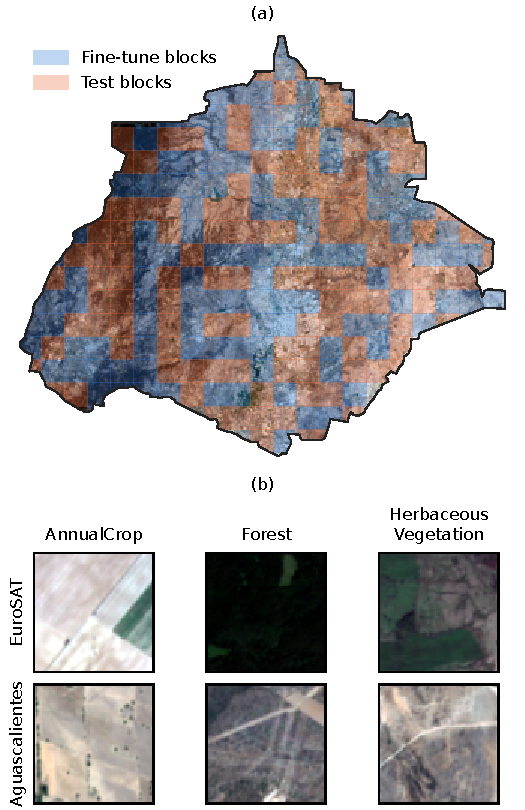
\includegraphics[width=\columnwidth]{study_area}
\caption{(a) April 2024 RGB composite of Aguascalientes with the 8$\times$8-cell blocks colored
by split (blue: fine-tune, orange: test) and the state outline. (b) One EuroSAT test patch (top
row) and one Aguascalientes test patch (bottom row) for AnnualCrop, Forest and
HerbaceousVegetation; they are the patches of the Grad-CAM figures. RGB stretch 2--98\,\% per
dataset; Aguascalientes uses the global limits of the composite, as the labeling previews did.
Note how differently the same class looks in Europe and in semi-arid Aguascalientes.}
\label{fig:study_area}
\end{figure}

\section{Methodology}\label{sec:methodology}

We trained three pre-trained models on EuroSAT under one shared protocol, tested them on
Aguascalientes without local training, and then fine-tuned them on the Aguascalientes fine-tune
split. This section describes the models, the protocol, the experiments and the metrics.

\subsection{Models and initialization}

We compared ResNet-50, a CNN whose layers learn residual functions;
EfficientNet-B0, the baseline of a CNN family scaled in depth, width
and resolution; and ViT-S/16, a pure transformer applied to a sequence
of 16$\times$16-pixel image patches. This gives two CNN families and one transformer that can
all be trained on one desktop machine with the same settings. We chose the small ViT because its
size is close to that of ResNet-50: with RGB input it has \ParamsViTRgb~M parameters against
\ParamsResNetRgb~M, while EfficientNet-B0 has \ParamsEffNetRgb~M (Table~\ref{tab:cost}). A CNN
versus ViT gap is therefore not just a gap in model size.

All three models started from ImageNet weights (timm). For ResNet-50 and
ViT-S/16 we also used SSL4EO-S12 weights~\cite{wang2023ssl4eo}, learned without labels on
the Sentinel-2 L1C images of the SSL4EO-S12 corpus with self-supervised methods that include MoCo
and DINO. We used the MoCo weights for ResNet-50 and the DINO weights for ViT-S/16. These
weights exist only for the 13 L1C bands, and they expect TorchGeo's normalization, $x/\num{10000}$. EfficientNet-B0 has no
SSL4EO-S12 weights, so it has only ImageNet runs. The SSL4EO-S12 band order puts B8A right after B08, while our data keep B8A
last. We therefore permuted the input channels of the first layer to EuroSAT order; without
this step, B8A and B09 to B12 would each enter through a filter learned for a different band.

ImageNet models expect three input channels, so the 13-band runs needed a new first layer (the
first convolution, or the patch embedding of the ViT). We copied the pre-trained RGB filters to
B04, B03 and B02 and set every other channel to the mean of the three. In this way, the RGB
filters stay exactly as pre-trained, and the new channels start from a neutral filter instead
of random noise that would disturb the pre-trained features in the first epochs.

\subsection{Shared training protocol}

The three models share everything except the architecture, as Table~\ref{tab:config} shows. We
never changed a hyperparameter for one model only, so that differences come from the
architecture and not from tuning. For example, if only the ViT had received a tuned learning
rate, a ViT advantage could be the result of that tuning. Patches were resized from 64 to
224~pixels because this is the input size of the pre-trained weights. ImageNet runs used the
per-band mean and standard deviation of EuroSAT train, also on Aguascalientes, so that no
statistic of the test region enters the pipeline. Every run used seed 0 and was trained once,
so we have no variance estimate across seeds.

\begin{table}[t]
\centering
\footnotesize
\caption{Configuration shared by every run, from the base configuration file. Only the architecture, the input bands and the initial weights change between runs.}
\label{tab:config}
\begin{tabular}{@{}lp{0.68\columnwidth}@{}}
\toprule
Setting & Value \\
\midrule
Input & 64$\times$64 resized to 224$\times$224 (bilinear) \\
Normalization & ImageNet: per-band mean and std of EuroSAT train; SSL4EO-S12: $x/\num{10000}$ (TorchGeo) \\
Augmentation & horizontal flip, vertical flip, 90$^\circ$ rotations \\
Optimizer & AdamW, lr \num{1e-04}, weight decay 0.05 \\
Schedule & 1 warmup epoch + cosine \\
Batch size & 64 (2$\times$32, accumulation) \\
Epochs (EuroSAT) & max 15, patience 3 on val macro-F1 \\
Loss & EuroSAT: cross-entropy; Aguascalientes: class-weighted cross-entropy \\
Fine-tuning & modes \texttt{head}, \texttt{last\_block}; 10 fixed epochs, last epoch kept \\
Seed & 0 \\
\bottomrule
\end{tabular}
\end{table}


We ran every experiment on the same Mac mini with an Apple M2 Pro, using the PyTorch MPS
backend in fp32. Because of memory, the effective batch of 64 was built from two micro-batches
of 32 with gradient accumulation; BatchNorm therefore saw 32 samples at a time.

\subsection{Experiments}

The study has four experiments. In E1 we trained the three models on EuroSAT with ImageNet
weights, each with RGB and with 13 bands (6 runs). In E2 we trained ResNet-50 and ViT-S/16 with
SSL4EO-S12 weights and 13 bands (2 runs). In E3 we evaluated the 8 resulting checkpoints on the
Aguascalientes test split without any local training, that is, zero-shot. In E4 we fine-tuned
the 8 checkpoints on the fine-tune split in two modes (16 runs). Because SSL4EO-S12 runs also
use a different normalization, a gap between SSL4EO-S12 and ImageNet runs cannot be credited to
the weights alone.

The two fine-tuning modes differ in how much of the network they train. In \texttt{head} mode,
the backbone was frozen and only the classifier was trained. In \texttt{last\_block} mode, the
last stage or block was trained together with the classifier. Frozen parts ran in evaluation
mode, so BatchNorm kept its EuroSAT statistics and dropout was off. To keep rare classes from
being ignored, the cross-entropy loss used the class weights
\begin{equation}
  w_c = \frac{n}{K\, n_c},
  \label{eq:class_weights}
\end{equation}
where $n$ is the number of fine-tune patches, $K$ is the number of classes and $n_c$ is the
number of fine-tune patches of class $c$. The weights came from the fine-tune split only.
Fine-tuning ran for a fixed 10 epochs and we kept the last epoch. We chose fixed epochs
because there is no validation split in Aguascalientes: early stopping on the test split would
leak test information into the model. One confound remains: \texttt{last\_block} trains a
different share of the parameters of each architecture, so a CNN versus ViT gap after
\texttt{last\_block} cannot be credited to the architecture alone.

\subsection{Metrics}

Our main metric is macro-F1, the average of the per-class F1 scores. With it, a rare class
counts as much as a common one; with accuracy, a model could score well on Aguascalientes by
predicting HerbaceousVegetation for most patches. The Aguascalientes macro-F1 averages the 9
classes with at least 10 test patches, so River is reported separately. We also report the
macro-F1 over all 10 classes and the accuracy. For cost, we recorded parameters, training time,
peak memory, inference throughput (patches/s) and the epochs needed to reach 95\,\% of the best
validation macro-F1.

To measure the domain shift, we defined the drop and the recovery as
\begin{align}
  \mathrm{Drop} &= \mathrm{F1}_{\mathrm{EuroSAT}} - \mathrm{F1}_{\mathrm{Ags}}^{\text{zero-shot}},
  \label{eq:drop}\\
  \mathrm{Recovery} &= \frac{\mathrm{F1}_{\mathrm{Ags}}^{\text{fine-tuned}}
    - \mathrm{F1}_{\mathrm{Ags}}^{\text{zero-shot}}}{\mathrm{Drop}},
  \label{eq:recovery}
\end{align}
where $\mathrm{F1}_{\mathrm{EuroSAT}}$ is the macro-F1 over the same 9 classes, computed from
the per-class F1 on the EuroSAT test set. In other words, the drop is what a model loses when
it moves to Aguascalientes, and the recovery is the fraction of that loss that fine-tuning wins
back. Recovery is undefined when $\mathrm{Drop} \le 0$.

We fixed the selection rule before seeing any result. The selected model is the one with the
highest Aguascalientes macro-F1 after \texttt{last\_block} fine-tuning. If two models are within
0.01 macro-F1, the one with the higher patches/s on the EuroSAT test set wins. Freezing the
rule first prevents choosing the criterion that favors a preferred model after the fact.

\subsection{Grad-CAM}

To see which parts of a patch drive a prediction, we used Grad-CAM~\cite{selvaraju2017}. We
computed it for the predicted class on the 224$\times$224 input, resized the map to the
64$\times$64 patch and scaled it to $[0, 1]$. The target layer was the last block of
\texttt{layer4} for ResNet-50 and \texttt{conv\_head} for EfficientNet-B0, the last
convolutional features of each CNN. For ViT-S/16 we used the first LayerNorm (\texttt{norm1})
of the last block. There, we dropped the CLS token and reshaped the 196 patch tokens into a
14$\times$14 map, so the gradients have a spatial layout. We chose this layer because it is the
last point where the patch tokens still affect the prediction: after the last attention layer,
only the CLS token reaches the classifier, so the gradients on the patch tokens would be zero.

\section{Experimental Results}\label{sec:results}

On EuroSAT the eight runs were almost tied; in Aguascalientes all of them lost most of their
macro-F1, and fine-tuning won back only part of it. We report the results in the order of the
experiments: EuroSAT, Aguascalientes without and with fine-tuning, the input and weight
variants, the cost, the selected model and the Grad-CAM maps. Every configuration was trained
once with seed 0, so we report the highest observed values and make no claim that one model is
better than another.

\subsection{EuroSAT}

All eight runs reached almost the same score on the EuroSAT test set. Table~\ref{tab:eurosat}
shows that macro-F1 ranged from \EuroSATMin{} to \EuroSATMax, and accuracy followed the same
pattern. ResNet-50/MS13/SSL4EO had the highest observed value in both columns. This means that
EuroSAT alone does not separate the models.

\begin{table}[t]
\centering
\footnotesize
\caption{EuroSAT test set (10 classes): overall accuracy and macro-F1 of the eight runs. Best value per column in bold.}
\label{tab:eurosat}
\begin{tabular}{lrr}
\toprule
Run & Accuracy & Macro-F1 \\
\midrule
ResNet-50 / RGB / ImageNet & 0.984 & 0.983 \\
ResNet-50 / MS13 / ImageNet & 0.985 & 0.985 \\
ResNet-50 / MS13 / SSL4EO & \textbf{0.993} & \textbf{0.993} \\
EfficientNet-B0 / RGB / ImageNet & 0.984 & 0.984 \\
EfficientNet-B0 / MS13 / ImageNet & 0.985 & 0.985 \\
ViT-S / RGB / ImageNet & 0.991 & 0.991 \\
ViT-S / MS13 / ImageNet & 0.990 & 0.990 \\
ViT-S / MS13 / SSL4EO & 0.987 & 0.987 \\
\bottomrule
\end{tabular}
\end{table}


The training curves tell the same story. Fig.~\ref{fig:convergence} shows the validation
macro-F1 per epoch: every run reached a high value within the first few epochs and changed
little afterwards. The curves differ mainly in the first epoch, where the two ResNet-50 runs
with ImageNet weights started lowest. With 13 bands, the SSL4EO-S12 run of each model started
higher than the ImageNet run of the same model, although ViT-S/RGB/ImageNet started slightly
above ViT-S/MS13/SSL4EO. The epochs needed to reach 95\,\% of the best validation macro-F1 did
not separate the models either: every run needed at most \EpochsToNinetyFiveMax{} epochs.

\begin{figure}[t]
\centering
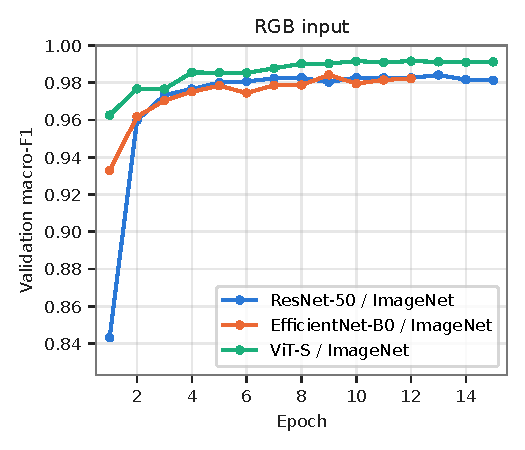
\includegraphics[width=\columnwidth]{convergence_rgb}\\[2pt]
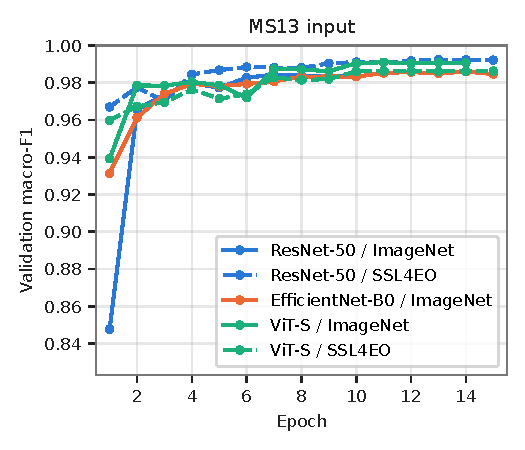
\includegraphics[width=\columnwidth]{convergence_ms13}
\caption{Validation macro-F1 on EuroSAT per training epoch. Top: RGB input. Bottom: 13-band
(MS13) input; dashed lines are the SSL4EO-S12 runs.}
\label{fig:convergence}
\end{figure}

\subsection{Aguascalientes without fine-tuning}

The models lost most of their EuroSAT performance when we tested them on Aguascalientes
without local training. The zero-shot column of Table~\ref{tab:ags} shows macro-F1 between
\ZeroShotMin{} and \ZeroShotMax{} over the nine classes. The drop, the EuroSAT F1 minus the
zero-shot F1, ranged from \DropMin{} to \DropMax. In other words, most of what the models
learned in Europe did not carry over to semi-arid Aguascalientes.

\begin{table*}[t]
\centering
\footnotesize
\caption{Macro-F1 on the Aguascalientes test split. The class set is the 9 classes with at least 10 test patches (1 class excluded and reported separately). EuroSAT F1 is the macro-F1 of the EuroSAT test result over the same classes. Drop = EuroSAT F1 minus zero-shot; recovery = (fine-tuned minus zero-shot) / drop, shown as -- when the drop is not positive. Best F1 per column in bold.}
\label{tab:ags}
\begin{tabular}{lrrrrrrr}
\toprule
Run & EuroSAT F1 & Zero-shot & Head & Last block & Drop & Rec. head & Rec. last block \\
\midrule
ResNet-50 / RGB / ImageNet & 0.983 & 0.259 & 0.308 & 0.278 & 0.724 & 0.068 & 0.026 \\
ResNet-50 / MS13 / ImageNet & 0.984 & 0.271 & 0.339 & 0.371 & 0.713 & 0.095 & 0.140 \\
ResNet-50 / MS13 / SSL4EO & \textbf{0.993} & \textbf{0.354} & 0.372 & \textbf{0.525} & 0.639 & 0.029 & 0.268 \\
EfficientNet-B0 / RGB / ImageNet & 0.984 & 0.271 & 0.275 & 0.400 & 0.713 & 0.006 & 0.181 \\
EfficientNet-B0 / MS13 / ImageNet & 0.984 & 0.196 & 0.217 & 0.361 & 0.788 & 0.027 & 0.209 \\
ViT-S / RGB / ImageNet & 0.991 & 0.326 & \textbf{0.380} & 0.441 & 0.665 & 0.081 & 0.173 \\
ViT-S / MS13 / ImageNet & 0.989 & 0.287 & 0.340 & 0.361 & 0.703 & 0.076 & 0.106 \\
ViT-S / MS13 / SSL4EO & 0.987 & 0.287 & 0.305 & 0.428 & 0.699 & 0.025 & 0.201 \\
\bottomrule
\end{tabular}
\end{table*}


Fig.~\ref{fig:ags_f1}(a) shows where the loss happened. HerbaceousVegetation had the highest
per-class F1 in every run, while Forest and Pasture were at or near zero in every run. River
appears hatched because it has only seven test patches and is reported separately. The pattern
is the same for the three architectures, both inputs and both kinds of weights.

\begin{figure*}[t]
\centering
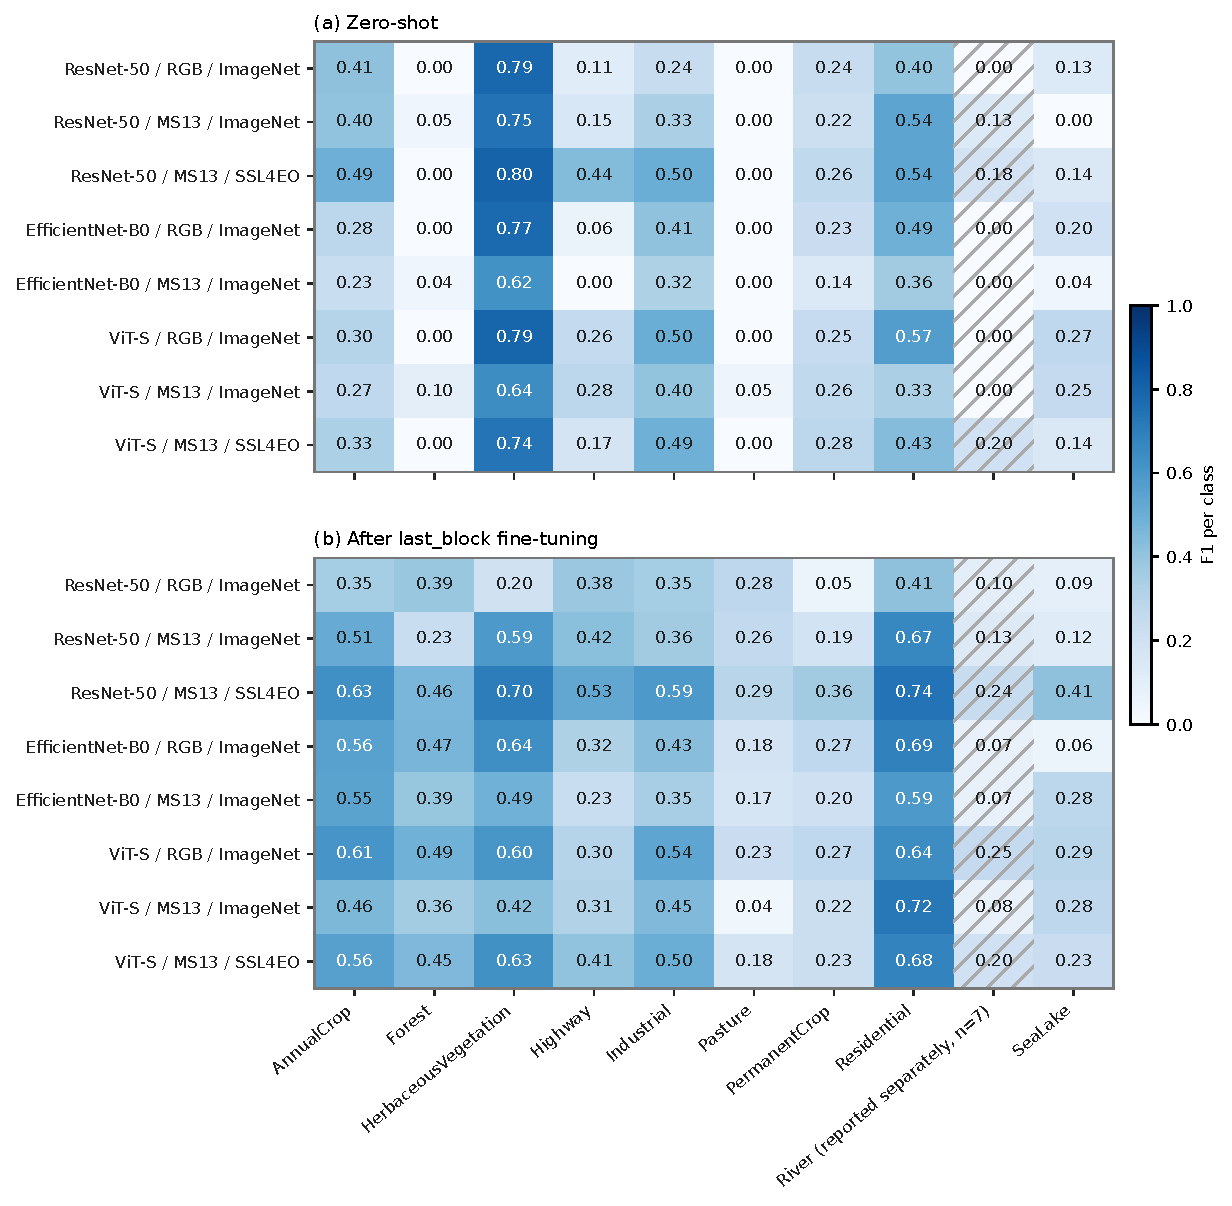
\includegraphics[width=0.75\textwidth]{ags_f1_per_class}
\caption{Per-class F1 on the Aguascalientes test split for the eight runs. (a) Zero-shot.
(b) After \texttt{last\_block} fine-tuning. River (hatched) has too few test patches and is
reported separately.}
\label{fig:ags_f1}
\end{figure*}

The confusion matrix shows the same collapse from the side of the predictions.
Fig.~\ref{fig:confusion}(a) gives the zero-shot confusion matrix of the model we selected later
(Section~\ref{sec:selected}). Most errors fell in the HerbaceousVegetation and PermanentCrop
columns; for example, every Forest test patch was predicted as HerbaceousVegetation. This means
that, without local training, the predictions concentrated in two classes, one of them the
largest class of the test set.

\begin{figure*}[t]
\centering
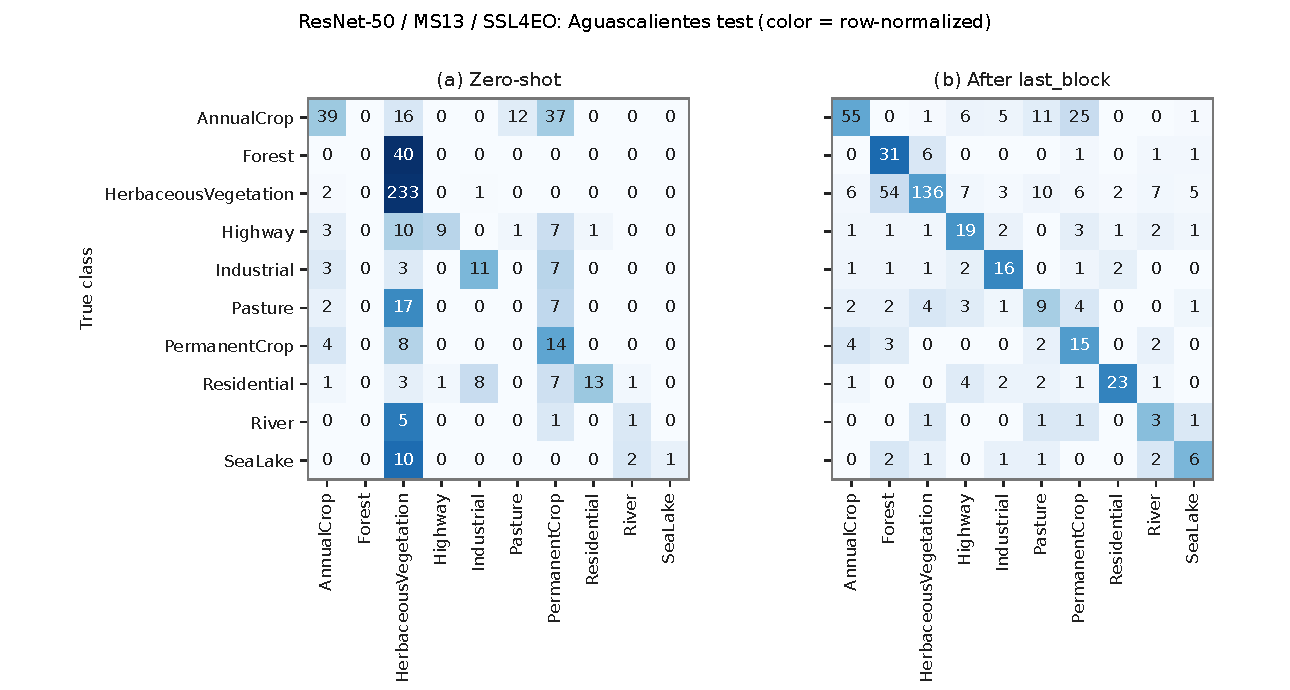
\includegraphics[width=\textwidth]{confusion_selected}
\caption{Confusion matrices of the selected model, ResNet-50/MS13/SSL4EO, on the
Aguascalientes test split. (a) Zero-shot. (b) After \texttt{last\_block} fine-tuning. Cells
show patch counts; the color is normalized per row (true class).}
\label{fig:confusion}
\end{figure*}

\subsection{Fine-tuning on Aguascalientes}

Fine-tuning won back only part of the drop, and how much depended on the mode. The Head and
Last block columns of Table~\ref{tab:ags} give the macro-F1 after each mode, and
Fig.~\ref{fig:drop_recovery} shows the drop (a) and the recovery (b) of every run. With
\texttt{head}, the recovery was at most \HeadRecoveryMax, so training only the classifier
barely changed the scores. With \texttt{last\_block}, the recovery ranged from \RecoveryMin{}
to \RecoveryMax. This means that the largest part of the drop remained after fine-tuning in
every run.

\begin{figure*}[t]
\centering
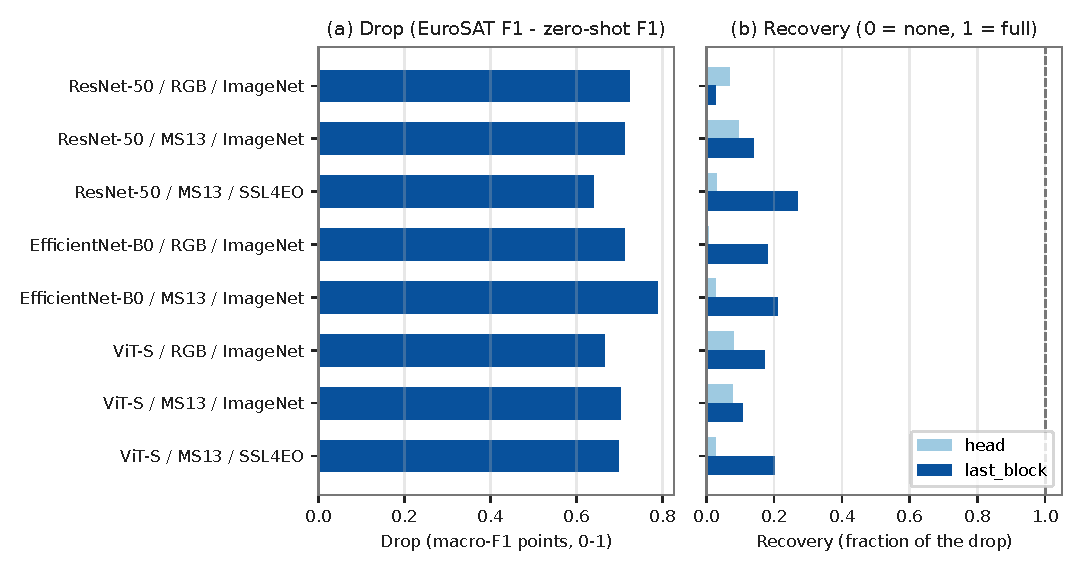
\includegraphics[width=\textwidth]{drop_recovery}
\caption{(a) Drop from EuroSAT macro-F1 to Aguascalientes zero-shot macro-F1 for each run.
(b) Recovery after \texttt{head} and \texttt{last\_block} fine-tuning, as a fraction of the
drop; the dashed line marks full recovery.}
\label{fig:drop_recovery}
\end{figure*}

One run did not follow the general order of the two modes. In every run except
ResNet-50/RGB/ImageNet, \texttt{last\_block} gave a higher macro-F1 than \texttt{head}. For
ResNet-50/RGB/ImageNet, macro-F1 after \texttt{last\_block} (\ResNetRgbLastBlock) was below
that after \texttt{head} (\ResNetRgbHead). Its Aguascalientes accuracy also fell, from
\ResNetRgbZeroShotAcc{} zero-shot to \ResNetRgbLastBlockAcc{} after \texttt{last\_block}.

The fall in accuracy was not limited to that run. In \AccuracyDropRuns{} of the \NumRuns{}
runs, \texttt{last\_block} lowered the Aguascalientes accuracy below its zero-shot value while
it raised macro-F1. This trade-off is consistent with the class-weighted loss of
Eq.~\eqref{eq:class_weights}, which shifts predictions away from the dominant
HerbaceousVegetation class. Fig.~\ref{fig:ags_f1}(b) shows both sides of it: Forest and Pasture
are no longer at zero in any run, and HerbaceousVegetation F1 is lower than zero-shot in every
run.

\subsection{Input bands and pre-trained weights}

Whether 13 bands helped depended on the model. Comparing the RGB and 13-band runs with ImageNet
weights in Table~\ref{tab:ags}, only ResNet-50 scored higher with 13 bands, both zero-shot and
after \texttt{last\_block}. EfficientNet-B0 and ViT-S scored lower with 13 bands in both
columns. In other words, our results do not support a general rule that more bands help under
this domain shift.

With 13 bands, the SSL4EO-S12 runs reached a higher macro-F1 after \texttt{last\_block} than
the ImageNet runs, for both ResNet-50 and ViT-S. Zero-shot, ResNet-50 was also higher with
SSL4EO-S12, while ViT-S gave the same value at three decimals with both kinds of weights. On
EuroSAT, ViT-S/MS13/SSL4EO was slightly lower than its ImageNet counterpart
(Table~\ref{tab:eurosat}). Because the SSL4EO-S12 runs also used a different normalization,
$x/\num{10000}$, these gaps cannot be credited to the weights alone. In the same way,
\texttt{last\_block} trains a different share of the parameters of each architecture, so we
leave the CNN versus ViT comparison after fine-tuning to Section~\ref{sec:discussion}.

\subsection{Computational cost}

Table~\ref{tab:cost} lists the cost of the eight EuroSAT runs. Peak memory is the memory
reserved by the MPS driver, not the memory that the weights and activations of the model need
on their own. ViT-S reserved the most: at least \PeakMemVitMin~GiB, against at most
\PeakMemCnnMax~GiB for the CNNs. Inference throughput ranged from \PatchesPerSecMin{} to
\PatchesPerSecMax{} patches/s, and each 13-band run had a lower throughput than the RGB run of
the same model.

\begin{table*}[t]
\centering
\footnotesize
\caption{Training cost of the eight EuroSAT runs on an Apple M2 Pro (fp32). Peak memory is the memory reserved by the MPS driver. Patches/s is inference throughput on the EuroSAT test set.}
\label{tab:cost}
\begin{tabular}{lrrrrr}
\toprule
Run & Params (M) & Train time (min) & Time/epoch (s) & Peak mem. (GiB) & Patches/s \\
\midrule
ResNet-50 / RGB / ImageNet & 23.5 & 58.3 & 233 & 4.31 & 208 \\
ResNet-50 / MS13 / ImageNet & 23.6 & 42.0 & 252 & 4.31 & 184 \\
ResNet-50 / MS13 / SSL4EO & 23.6 & 62.9 & 252 & 4.31 & 183 \\
EfficientNet-B0 / RGB / ImageNet & 4.0 & 45.5 & 227 & 4.33 & 233 \\
EfficientNet-B0 / MS13 / ImageNet & 4.0 & 57.8 & 231 & 4.33 & 214 \\
ViT-S / RGB / ImageNet & 21.7 & 54.6 & 218 & 5.18 & 236 \\
ViT-S / MS13 / ImageNet & 22.7 & 55.3 & 237 & 5.25 & 199 \\
ViT-S / MS13 / SSL4EO & 22.7 & 59.3 & 237 & 5.25 & 199 \\
\bottomrule
\end{tabular}
\end{table*}


Total training time is a weak basis for comparison, because early stopping ended the runs at
different epochs (Fig.~\ref{fig:convergence}). Time per epoch is the comparable column, and it
was similar across the three models. EfficientNet-B0 has far fewer parameters than ResNet-50 and
ViT-S, yet its time per epoch was close to theirs. This means that, on our hardware, the number
of parameters did not predict the training time.

\subsection{Selected model}\label{sec:selected}

Applying the selection rule fixed in Section~\ref{sec:methodology}, we selected
ResNet-50/MS13/SSL4EO with \texttt{last\_block} fine-tuning. Its Aguascalientes macro-F1 was
\AgsLastBlockBest, \SelectionMargin{} above the runner-up, which is wider than the tie-break
margin, so the throughput rule was not needed. Since only ResNet-50 and ViT-S have SSL4EO-S12
runs, we also applied the rule to the six ImageNet runs as a secondary result, where the three
models compete on equal weights. There, ViT-S/RGB/ImageNet came first with
\ImageNetLastBlockBest, \ImageNetSelectionMargin{} above the next run, again without a
tie-break.

Fig.~\ref{fig:confusion}(b) shows the selected model after \texttt{last\_block}. Compared with
panel (a), the predictions now spread along the diagonal instead of piling up in the
HerbaceousVegetation column. The largest off-diagonal cell is HerbaceousVegetation predicted as
Forest. In other words, the main error changed direction: from most patches being called
HerbaceousVegetation to part of HerbaceousVegetation being called Forest.

\subsection{Grad-CAM}

Fig.~\ref{fig:gradcam} shows the Grad-CAM maps of the RGB ImageNet run of each model, without
fine-tuning, on EuroSAT (a) and Aguascalientes (b). We drew one test patch per class at random
with seed 0, for six classes, so the patches were not chosen to make a point; the list and the
rule are stored with the figures. Under each map is the predicted class, marked as correct or
wrong. On EuroSAT all predictions but one are correct, while on Aguascalientes most are wrong,
and most of the wrong ones are HerbaceousVegetation.

\begin{figure*}[t]
\centering
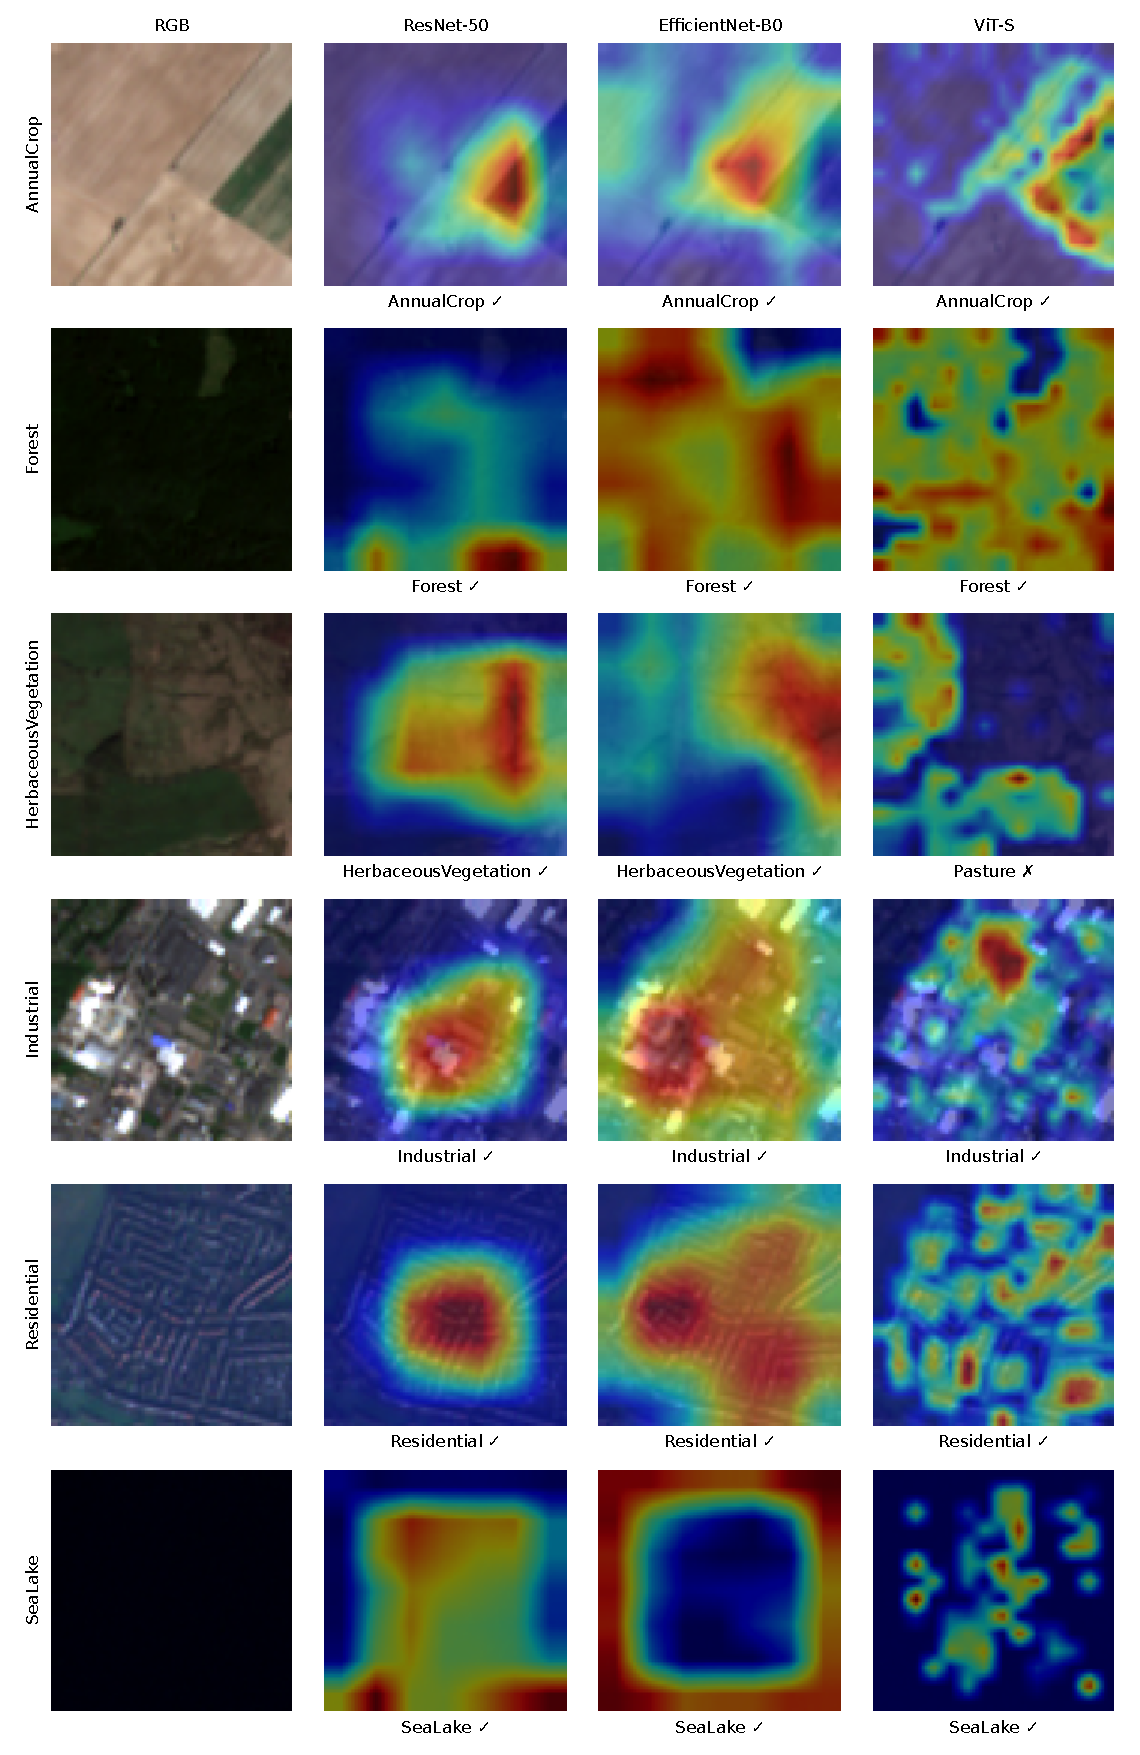
\includegraphics[width=0.48\textwidth]{gradcam_eurosat}\hfill
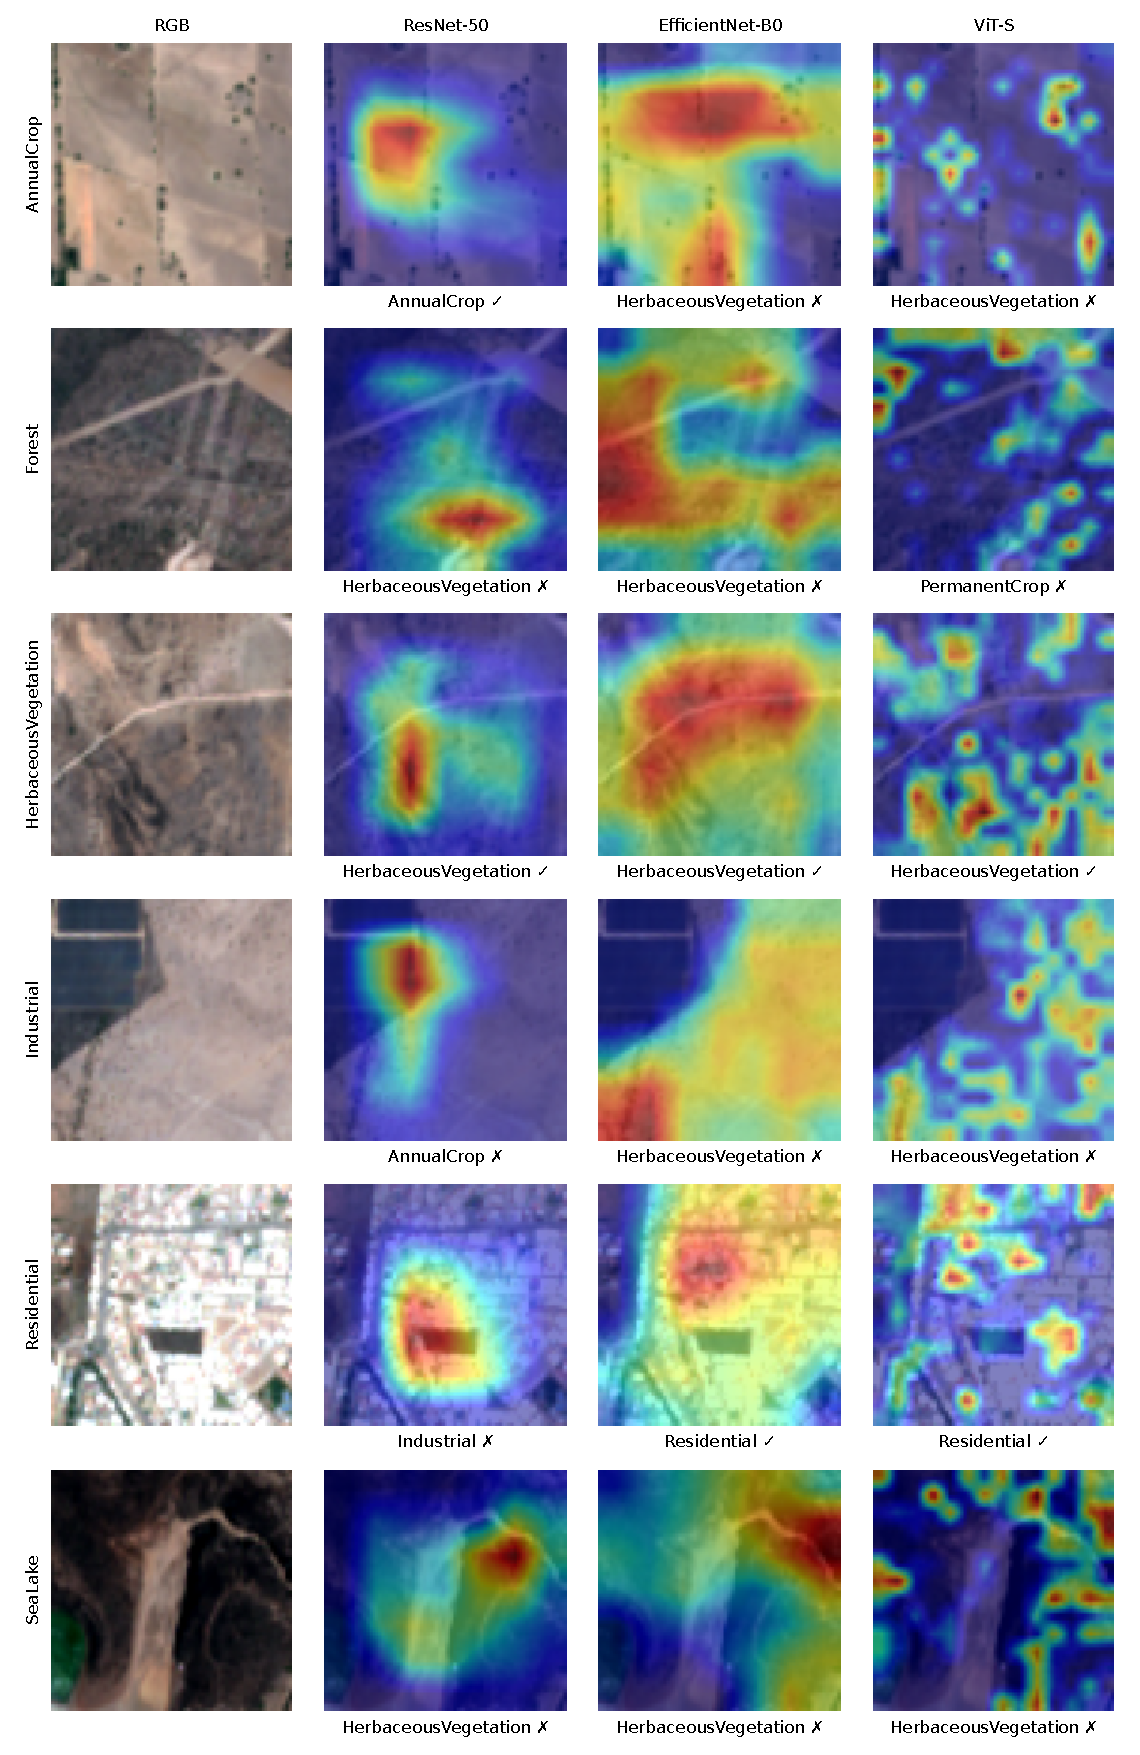
\includegraphics[width=0.48\textwidth]{gradcam_ags}
\caption{Grad-CAM maps of the RGB ImageNet runs, without fine-tuning, on one random test patch
per class (seed 0). (a) Left: EuroSAT. (b) Right: Aguascalientes. Columns: RGB patch,
ResNet-50, EfficientNet-B0 and ViT-S. Under each map: the predicted class, with a check mark if
correct and a cross if wrong.}
\label{fig:gradcam}
\end{figure*}

The two families of models produce maps of a different shape. CNN maps are smooth and
concentrated on one compact region of the patch, sometimes two. ViT-S maps are made of many
small spots spread over the whole patch. In Aguascalientes, many maps fall away from the object
that defines the class. The Industrial cell of Fig.~\ref{fig:gradcam}(b) is a solar park,
seen as a dark rectangle of panels at the top left. The maximum of the ResNet-50 map lies on
the edge of the panels. The maximum of EfficientNet-B0 falls in the lower-left corner, and the
spots of ViT-S spread over the bare ground. None of the three models predicted Industrial for
this patch.

Fig.~\ref{fig:gradcam_selected} compares the selected model before and after
\texttt{last\_block} on the Aguascalientes patches of Fig.~\ref{fig:gradcam}(b). The
HerbaceousVegetation and SeaLake rows are replaced by two HerbaceousVegetation patches drawn at
random with seed 0 among those that the fine-tuned model predicts as Forest; that is, they were
chosen to show the main error of Fig.~\ref{fig:confusion}(b). Both were correct zero-shot and
became Forest after \texttt{last\_block}. The AnnualCrop patch changed from a wrong prediction
to a correct one, the Forest and Industrial patches stayed wrong, and the Residential maps are
almost the same before and after. We leave the interpretation of all these maps to
Section~\ref{sec:discussion}.

\begin{figure*}[t]
\centering
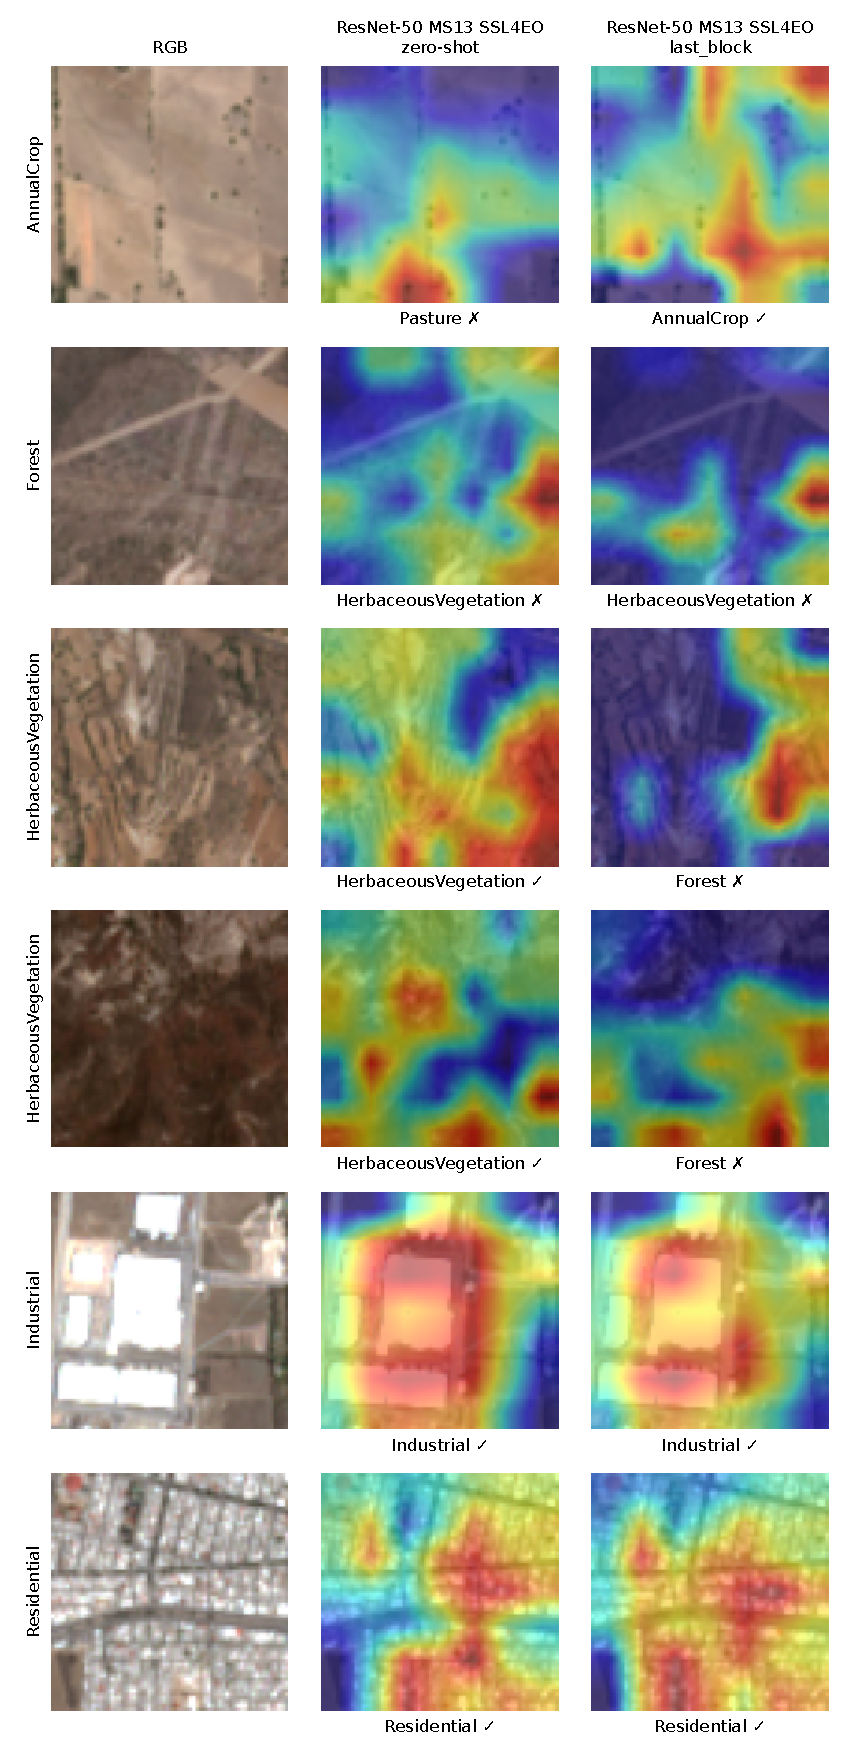
\includegraphics[height=0.5\textheight]{gradcam_selected}
\caption{Grad-CAM maps of the selected model, ResNet-50/MS13/SSL4EO, on Aguascalientes test
patches. Columns: RGB patch, zero-shot and after \texttt{last\_block}. The two
HerbaceousVegetation rows are random patches (seed 0) among those predicted as Forest after
\texttt{last\_block}; the other rows are the patches of Fig.~\ref{fig:gradcam}(b).}
\label{fig:gradcam_selected}
\end{figure*}

\section{Discussion}\label{sec:discussion}

\todo{Interpretation per research question, Grad-CAM evidence, limitations: one seed, small test set, single month (April 2024), 64-px patches, no SSL weights for EfficientNet, 541 test / 561 fine-tune patches; River (7 test patches) reported separately and excluded from macro-F1; 35 of the 541 test patches border a fine-tune cell across a block edge because the split has no buffer zone. Target length: 1 page.}

\section{Conclusions}\label{sec:conclusions}

Our goal was to measure how much a land-use classifier trained on EuroSAT loses in semi-arid
Aguascalientes, and how much of that loss light fine-tuning on local labels wins back. We
compared ResNet-50, EfficientNet-B0 and ViT-S/16 under one shared protocol, and three findings
stand out.

\begin{enumerate}
  \item \emph{The models were almost tied on EuroSAT, but all of them dropped sharply in
  Aguascalientes (RQ-a, RQ-b).} EuroSAT macro-F1 ranged from \EuroSATMin{} to \EuroSATMax, and
  without local training the drop ranged from \DropMin{} to \DropMax. This means that a
  near-perfect EuroSAT score does not guarantee a useful model in another region; the model has
  to be evaluated on local labels.
  \item \emph{Light fine-tuning won back only part of the drop (RQ-c).} Training the classifier
  alone (\texttt{head}) recovered at most \HeadRecoveryMax{} of the drop, and our runs cannot
  tell whether the features were too weak or the classifier was undertrained. Fine-tuning the
  last block (\texttt{last\_block}) recovered between \RecoveryMin{} and \RecoveryMax{}
  (Eq.~\ref{eq:recovery}). This means that most of the drop remained in every run after
  fine-tuning.
  \item \emph{The effect of the input bands and the weights depended on the model (RQ-d,
  RQ-e).} With ImageNet weights, 13 bands helped only ResNet-50 in Aguascalientes. With 13
  bands, the SSL4EO-S12 runs gave the highest observed macro-F1 after \texttt{last\_block} for
  both ResNet-50 and ViT-S, but they also used another normalization, so the gap cannot be
  credited to the weights alone. This means that the answer depends on the combination of model, bands and weights, not
  only on CNN versus ViT.
\end{enumerate}

The selection rule, fixed before any result, chose ResNet-50/MS13/SSL4EO with
\texttt{last\_block} fine-tuning, with a macro-F1 of \AgsLastBlockBest, \SelectionMargin{} above
the runner-up. Among the six ImageNet runs, where the three models compete on equal weights,
ViT-S/RGB/ImageNet came first with \ImageNetLastBlockBest, \ImageNetSelectionMargin{} above the
next run. On cost (RQ-a), EfficientNet-B0 had far fewer parameters but a similar time per epoch,
and ViT-S/RGB/ImageNet had the highest observed throughput, \PatchesPerSecMax{} patches/s.

What we learned is that the domain shift outweighed the differences between the models, so a
model for a new region has to be judged on local labels and a spatially separated test set, not
on EuroSAT alone. The selected model is the starting point for the second stage of the
project, a monthly land-use monitor of the state. Section~\ref{sec:discussion} lists the
experiments that would make these answers firmer.


\bibliographystyle{IEEEtran}
\bibliography{references}

\end{document}
